%
% ---------- header -----------------------------------------------------------
%
% project       kaneton
%
% license       kaneton
%
% created       julio guerra   [wed jun 10 20:54:07 2015]
%
%
% ---------- setup ------------------------------------------------------------
%

%
% path
%

\def\path{../../..}

%
% template
%

%
% ---------- header -----------------------------------------------------------
%
% project       kaneton
%
% license       kaneton
%
% file          kaneton/view/template/examclass.tex
%
% created       julio guerra   [sat mar 22 12:33:00 2014]
% updated       julio guerra   [sat mar 23 17:31:00 2014]
%

\input{.dependency.tex}

%
% document
%

\documentclass[a4paper,addpoints,10pt]{exam}
\extrawidth{1in}
\usepackage[utf8]{inputenc}

%
% header & footer
%

\pagestyle{headandfoot}
\headrule
\lhead{\school}
\chead{\class}
\rhead{\examdate}
\cfoot{\thepage/\numpages}

%
% exam class customization
%

\qformat{{\large \textbf{\thequestion\ -\ \thequestiontitle}} \droptotalpoints}
\totalformat{(\totalpoints\ points)}
\renewcommand{\thequestion}{\Roman{question}}
\renewcommand{\thepartno}{\arabic{partno}}
\renewcommand{\thesubpart}{\alph{subpart}}
\renewcommand{\partlabel}{\thepartno)}
\renewcommand{\subpartlabel}{(\thesubpart)}
\bonuspointpoints{point \textbf{bonus}}{points \textbf{bonus}}

%
% \gradingtable
%   print the point table if in printanswers mode
%
\newcommand{\gradingtable}
  {
    \ifprintanswers
      \newpage
      \begin{center}
        \combinedgradetable[v]
      \end{center}
    \fi
  }

%
% enable answers if compiling in private mode
%
\ifthenelse
  {
    \equal{\mode}{private}
  }
  {%
    \printanswers
  }
  {
  }


\usepackage{graphicx}
\usepackage{float}

\newcommand{\class}{EPITA\_ING2\_2016\_S4 NSE Julio Guerra}
\newcommand{\examdate}{2015}
\newcommand{\timelimit}{3h}
\newcommand{\school}{EPITA}

%
% exam
%
\begin{document}

%
% cover header
%

\begin{center}
  {\LARGE Noyaux et Systèmes d'Exploitation}\\
  \vspace{1cm}
  \textbf{Durée: 3 heures}\\
  \textbf{Documents et calculatrices interdits}\\
  \scriptsize{Sauf mention du contraire, toute réponse doit être justifiée, aucun point ne sera attribué sinon.}\\
  \scriptsize{Le nombre de points d'une question est uniquement fonction de son importance et n'est pas lié au nombre de réponses attendues.}\\
  \scriptsize{Une copie bien présentée sera toujours mieux notée.}\\
  \scriptsize{Les questions bonus donnent des points sommés à la note finale du partiel.}
\end{center}
\vspace{1cm}

%
% ---------- questions --------------------------------------------------------
%

\begin{questions}

%
% events
%
\titledquestion{Gestion des événements}
Pour chacun des événements suivants, répondre aux questions:
\begin{itemize}
  \item L'événement est-il synchrone ou bien asynchrone?
  \item Quel état faut-il sauvegarder/restaurer?
  \item Qui doit sauvegarder/restaurer cet état?
\end{itemize}
Les réponses doivent être générales, sans référence à une architecture particulière.

\begin{parts}
  % q
  \part[4] Un appel de fonction.
  \begin{solution}
  Procedure calls are synchronous. The caller saves the instruction pointer and the callee restores it (possibly with hardware assistance). The callee and the callee cooperate to save and restore the stack pointer, and the caller or the callee must agree on who saves other registers, but details vary.
  \end{solution}

  % q
  \part[4] Un appel système (syscall).
  \begin{solution}
  The transition between user and kernel privilege level needs hardware assistance, and there may be an address space change, but otherwise this is the same as (a).
  \end{solution}

  % q
  \part[4] Un changement de processus suite à l'expiration de son quantum de temps (time slice).
  \begin{solution}
Timer interrupts are asynchronous. The instruction pointer, stack pointer, and other registers, as well as any other process-visible state such as the current address space, must be saved by the kernel on behalf of the old process/thread and restored by the kernel on behalf of the new process/thread.
There is no caller or callee here, just old and new processes or threads.
  \end{solution}
\end{parts}

%
% processus
%
\titledquestion{Modèle des processus}
Soit un modèle de processus simple comprenant trois états: prêt, bloqué et élu.
\begin{parts}
  % q
  \part[4] Représenter le graphe d'état d'un processus.
  \begin{solution}
  Running -2-> <-1- Ready
  Blocked -3->      Ready
  Blocked -5->      Running
  \end{solution}

  % q
  \part[4] Légender le graphe en expliquant brièvement chaque transition.
  \begin{solution}
  Arrow 1: Process is scheduled and run by the scheduler.
  Arrow 2: Time slice runs out, but process is still wanting to run. Yield().
  Arrow 3: I/O completes, or lock is acquired. Woken up by a semaphore or conditional.
  Arrow 5: Any blocking action. I/O request, lock blocks.
  \end{solution}
\end{parts}

%
% Ordonnancement
%
\titledquestion{Ordonnancement}
Brièvement, donner les avantages et les inconvénients des algorithmes d'ordonnancement suivants:

\begin{parts}
  % q
  \part[2] Premier Arrivé Premier Servi (First-In First-Out).
  \begin{solution}
  Pro: Trivial. Con: Convoy effect, avg time to completion is very bad.
  \end{solution}

  % q
  \part[2] Tourniquet (Round-Robin).
  \begin{solution}
  Pro: Simple to implement, fair. Con: Avg time to completion for lots of large jobs is worst case.
  \end{solution}

  % q
  \part[2] Plus court d'abord.
  \begin{solution}
  Pro: Theoretically best. Con: Future prediction required. Unfair to long jobs.
  \end{solution}

  % q
  \part[2] Aléatoire.
  \begin{solution}
  Pro: Simple, Easy to do priority donation, very hard to “cheat” or drive system to bad behaviors. Con: Only fair in theory, jobs may never actually run.
  \end{solution}
\end{parts}

%
% Working set
%
\titledquestion{Working Set}
Soit NachOS, un système d'exploitation général implémentant:
\begin{itemize}
  \item une gestion de la mémoire virtuelle paginée sur demande (demand paging) avec va-et-vient (swapping).
  \item une politique de remplacement de page locale au processus\footnote{Le remplacement est local au processus lorsque la page évincée est choisie parmi celles du processus, tandis qu'un remplacement global opère sur les pages de tous les processus.} (local replacement policy) lorsqu'il n'y a plus d'espace disponible en mémoire principale (RAM).
  \item un ordonnancement de processus avec priorité.
\end{itemize}
Soient deux processus non-intéractifs (CPU-bound) A et B dont les ensembles de travail\footnote{On appelle ensemble de travail l'ensemble des pages utilisées pendant un certain temps par un processus.} (working sets) sont respectivement de 50Go et 100Mo.\\\\
Le système d'exploitation exécute A et B sur un système monoprocesseur avec 1Go de mémoire principale et 300Go de mémoire de masse auxiliaire.

\begin{parts}
  % q
  \part[2] Pourquoi et comment les ordonnanceurs avec priorité des systèmes généraux tendent à favoriser les tâches intéractives?

  % q
  \part[4] Quel processus se voit attribuer ici la priorité la plus haute?
  \begin{solution}
  Job A will have a CPU scheduling priority higher than Job B. In fact, Job A's Working Set (50 GB) is much higher than the memory (1 GB); even if it is supposed to be a compute-intensive job, it will spend most of its time doing I/O operations to bring in pages it needs never finishing its time slice. Therefore, according to the priority scheduler, Job A's priority is raised. On the contrary, Job B's Working Set (100 MB) can easily fit in memory, and will be assigned lower priority by the priority scheduler.
  \end{solution}
  % q
  \part[4] Comment l'ajout d'un deuxième cœur affecte-t-il les priorités de A et B?
  \begin{solution}
  When you add a second CPU, the priority concept loses some significance since both jobs could run in parallel on those CPUs. However, the priority relation between Job A and Job B remains the same: namely, Job A priority stays higher than Job B's. Adding a second CPU would not really change the scenario much in priority terms: Job A is still doing plenty of I/O operations as before (priority boosted), and Job B can still easily fit in memory (priority lowered, since it's a compute-intensive job).
  \end{solution}

  % q
  \part[2] Comment une politique de remplacement de page global affecte-t-il les priorités de A et B?
  \begin{solution}
    Job A can now evict Job B's pages. This means that Job A has a chance to run longer (more pages in memory, fewer page faults), and its priority may lower a little. Job B will instead see its priority boosted: having its pages taken away by Job A, causes Job B to perform I/O operations to bring in its pages. Therefore, Job B's priority raises.
  \end{solution}
\end{parts}

%
% mmu
%
\titledquestion{Unité de gestion de la mémoire}
L'unité de gestion de la mémoire (Memory Management Unit (MMU)) de l'architecture 32 bits Intel (IA32) combine la segmentation puis la pagination.
Le schema suivant illustre de manière simplifiée (et suffisante pour cet exercice) la MMU de cette architecture. On ignorera tout au long de l'exercice la segmentation.

\begin{figure}[H]
  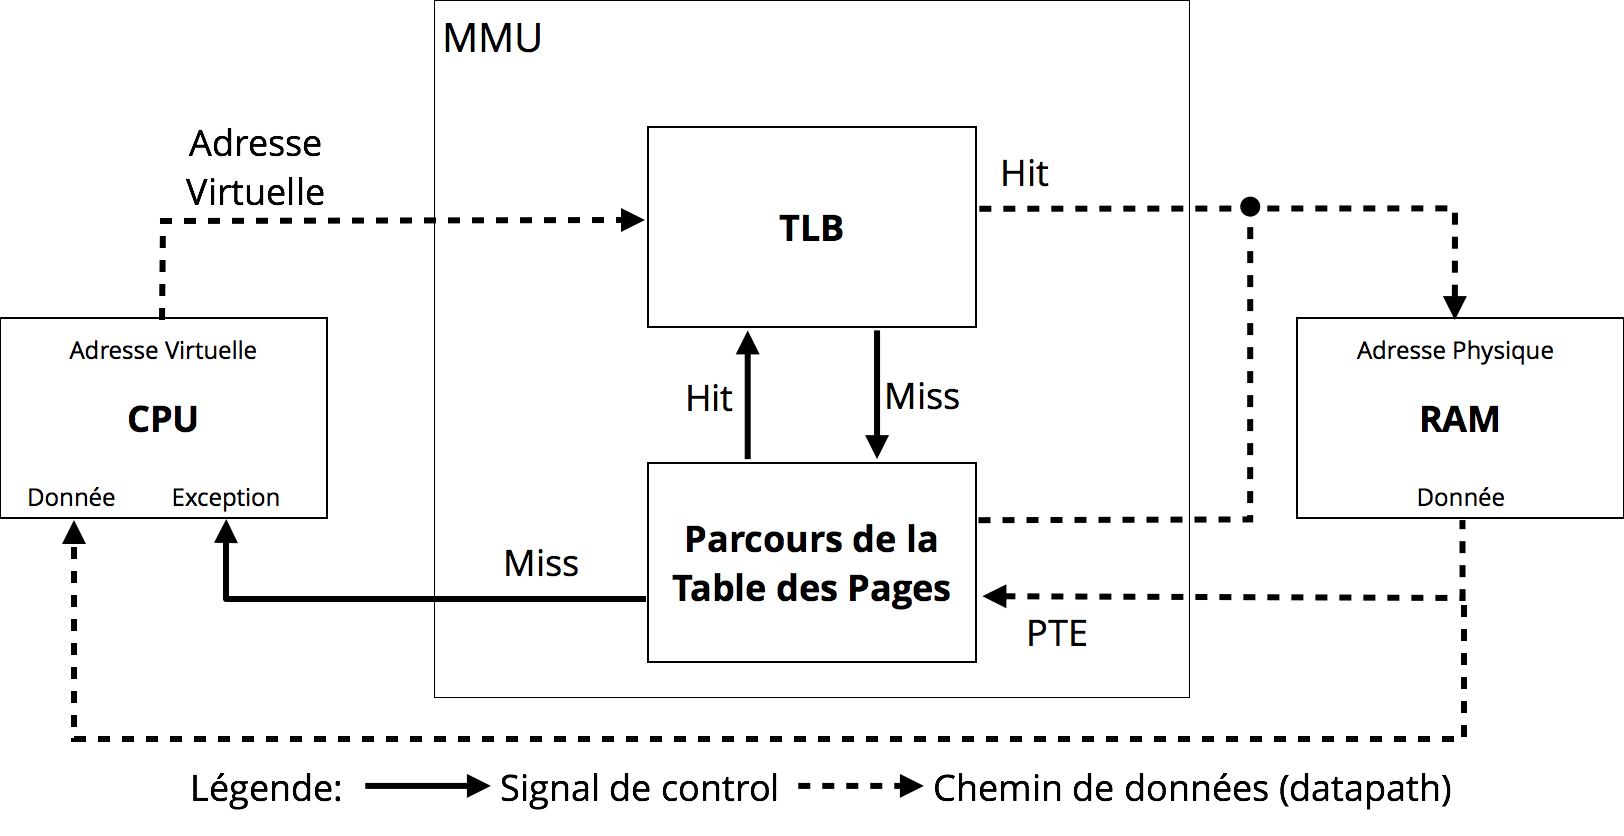
\includegraphics[width=\linewidth]{mmu}
\end{figure}

La table des pages a deux niveaux (two-level page tables) et est gérée par le système d'exploitation en RAM. Le reste de la translation d'adresse est automatiquement géré par le processeur: parcours de la table des pages matériel assisté d'un Translation Lookaside Buffer (TLB) simplement indexé par les adresses virtuelles de l'espace d'adressage courant (lors d'un changement de contexte processus, le TLB est vidé).

\begin{parts}
  \part Décrire brièvement les mécanismes matériels et logiciels ayant lieu lorsqu'un processus utilisateur fait un accès mémoire pour chacun des cas suivants:
  \begin{subparts}

  % q
  \subpart[1] L'adresse fait partie de l'espace d'adressage du processus et est présente en mémoire principale (RAM).
  \begin{solution}
  Segment 0xD, Page 0xEADB, Offset 0xEEF. Lookup the base/bound and where the page table is for segment 0xD. Check them all for validity. Look at the 0xEADB’th PTE (0xEEF * 4 bytes into the page table) and see what physical page it is in. Add 0xEEF to that physical page number shifted 12 bits to the left. Access memory. Hopefully all that was in the TLB, so it’s all cached in the hardware.
  \end{solution}

  % q
  \subpart[1] L'adresse fait partie de l'espace d'adressage du processus et est présente en mémoire de masse auxiliaire.
  \begin{solution}
  If it is paged out to disk, when you look at the PTE, instead of a physical page number you will see the present bit un-set and a disk offset/pointer to the page on disk, and generate a page fault. The OS then requests that block to be loaded in, and puts the thread on the blocked list. When the page is returned by the I/O device, a physical page is allocated, the block put there, the PTE present bit is set and the physical page number set. The thread is then put on the ready list, and the instruction restarted.
  \end{solution}

  % q
  \subpart[1] L'adresse ne fait pas partie de l'espace d'adressage du processus.
  \begin{solution}
  At any of the steps in part A) we could find an invalid PTE, an address out of bounds etc. In which case the process would raise a page fault, and since it’s not valid, probably be killed.
  \end{solution}
  \end{subparts}

  \part[5] Donner un exemple d'accès mémoire entraînant exactement deux TLB miss en cascade. Les hypothèses de la question suivante peuvent aider.

  \part[6] Décrire le pire cas d'accès mémoire possible à une adresse par un processus.\\
  Pour simplifier cette analyse, supposer:
  \begin{itemize}
  \item Le système d'exploitation sur lequel le processus s'exécute implémente une gestion de la mémoire paginée (demand paging) avec va-et-vient (swapping).
  \item Le TLB est plein d'adresses de l'espace utilisateur du processus\footnote{Ce cas peut arriver si aucune interruption ni préemption ni appel système n'ont lieu durant l'exécution du processus et que le processus a un working set associé est supérieur à la capacité du TLB.}.
  \item La totalité des pages noyau sont présentes en mémoire principale (RAM) et ne peuvent pas en être évincées ou remplacées.
  \item Les pages noyau ne sont pas protégées dans le TLB, elles peuvent en être évincées.
  \item Le working set du processus est supérieur à l'espace RAM disponible.
  \item La gestion d'un va-et-vient de page (page swapping) a un working set supérieur à la capacité du TLB.
  \end{itemize}

    % q
  \bonuspart[2] En déduire l'équation du pire temps d'exécution d'une lecture mémoire.
\end{parts}

%
% multiprogrammation
%
\titledquestion{Modèle de Multiprogrammation}
Soit un système \textbf{monoprocesseur} taillé sur mesure pour exécuter le système d'exploitation multitâche coopératif WesterOS (cooperative multitasking), un système d'exploitation multi-processus et multi-thread. La nouvelle version de WesterOS introduit le multitâche préemptif (preemptive multitasking) pour tous les processus.

\begin{parts}
  \part Cette transition pose problème aux programmes existants qui ont faits le postulat de s'exécuter sur un système d'exploitation avec un ordonnancement coopératif, c'est-à-dire sans préemption.
  \begin{subparts}
    % q
    \subpart[4] Quel problème peut désormais survenir pour les programmes existants?

    % q
    \subpart[2] Quelle modification doivent subir les programmes existants?
    \begin{solution}
    Threads and processes in a cooperative multitasking environment have little need for explicit synchronization. Every sequence of code between calls to yield() (or other functions that block) is implicitly a critical section. If preemptive multitasking is introduced, applications must be modified to use explicit synchronization.
    \end{solution}

    % q
    \subpart[2] Dans quel cas les programmes existants ne nécessitent aucun changement?
    \begin{solution}

    \end{solution}
  \end{subparts}

  % q
  \part[4] Quelle est le seul prérequis matériel pour permettre la préemption?
  \begin{solution}
  A system with preemptive multitasking needs a periodic timer interrupt to enforce time slicing.
  The machine is still a uniprocessor machine, so atomic compare and swap instructions, etc., are not needed for synchronization.
  \end{solution}
\end{parts}

%
% SMP
%
\titledquestion{Symmetric Multiprocessing}
\begin{parts}
  % q
  \part[2] Définir Symmetric Multiprocessing (SMP).

  \part Pour chacun des cas suivants, quelle raison précise amène à limiter le nombre de threads concurrents:
  \begin{subparts}
  % q
  \subpart[2] La taille des caches.

  % q
  \subpart[2] La taille de la mémoire principale.

  % q
  \subpart[2] La bande passante des entrées/sorties.

  % q
  \subpart[2] L'overhead des synchronisations interthread.
  \end{subparts}

  \part Soit le système d'exploitation PollOS taillé sur mesure pour une machine monoprocesseur.\\
  Vous êtes l'architecte de sa prochaine version qui se doit de supporter le SMP comme son concurrent HermanOS.
  \begin{subparts}
  % q
  \subpart[4] Que faut-il globalement éviter afin de produire un bon système SMP?

  % q
  \subpart[2] Donner trois nouvelles fonctionnalités matérielles nécessaires?

  % q
  \subpart[2] Donner trois ajouts/modifications logiciels nécessaires?
  \end{subparts}
\end{parts}

%
% virtualisation
%
\titledquestion{Virtualisation}
\begin{parts}

  % q
  \part La virtualisation a pour philosophie d'intercepter toute exception et instruction privilégiée en forçant une transition vers l'hyperviseur.
  \begin{subparts}
    \subpart Dans le cas \textbf{sans} support matériel de virtualisation:
      \begin{subsubparts}
        % q
        \subsubpart[1] Donner un exemple d'instruction privilégiée à intercepter.

        % q
        \subsubpart[2] Dessiner et expliquer brièvement le flot de contrôle (control-flow) d'un appel système fait par une application s'exécutant sur l'OS guest.

        % q
        \subsubpart[1] Quel est l'inconvénient majeur de ce mode d'hypervision?
      \end{subsubparts}

      % q
      \subpart Dans le cas \textbf{avec} support matériel de virtualisation:
      \begin{subsubparts}
        % q
        \subsubpart[1] Quel est l'ajout majeur au matériel permettant de supporter la virtualisation?

        % q
        \subsubpart[2] Dessiner et expliquer brièvement le flot de contrôle (control-flow) d'un appel système d'une application s'exécutant sur l'OS guest.

        % q
        \subsubpart[1] Quel est l'avantage majeur de ce mode d'hypervision?

      \end{subsubparts}
  \end{subparts}

\end{parts}

\end{questions}

%
% grading table
%
\gradingtable

\end{document}
